
\section{Data}
The dataset was obtained from kaggle\cite{imet}.
It contains 109,237 images of museum artifacts from the Metropolitan Museum of Art in New York.
The exact source of the images is unknown.
All objects have been labeled by  annotators without verification, thus noisy data is to be expected.
Each annotator was asked to label what he sees in the image.
Labels can describe what culture this object belongs too, or what the object was used for.
For example the image in figure \ref{fig:1} was annotated with: german, nymphenburg, children, female nudes and utilitarian objects.
Figure \ref{fig:2} shows some more example data.
\begin{figure}[h]
    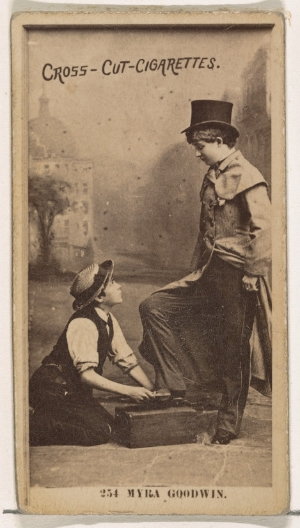
\includegraphics[width=0.33\textwidth]{images/1}
    \caption{An teapot}
    \label{fig:1}
\end{figure}
Furthermore 7,443 images are available for verification.
Both the training and verification image-sets have an corresponding csv-file where one row corresponds with one image.
The images are labeled using numbers, an additional csv-file is given containing the corresponding attributes for each number.
There are 1103 labels in total.
\begin{figure}[h]
    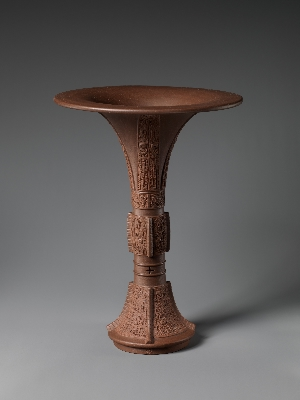
\includegraphics[width=.2\textwidth]{images/3}
    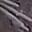
\includegraphics[width=.2\textwidth]{images/4}
    \caption{Example images from the dataset}
    \label{fig:2}
\end{figure}
